\section{Ejercicio 2: Heurística constructiva golosa}

  % \begin{figure}[ht]
  %   \begin{center}
  %     \includegraphics[width=0.5\columnwidth]{imagenes/pacman.png}
  %     \caption{Perdidos y con poca fuerza}
  %   \end{center}
  % \end{figure}

    % 1. Describir detalladamente el problema a resolver dando ejemplos del mismo y sus soluciones.
    \subsection{Descripción del problema y solución propuesta}
        En este punto, se pidió realizar un algoritmo basado en una heurística constructiva golosa que resuelva el problema en cuestión. El mismo al tratarse de una heurística puede no dar la solución óptima, y puede no devolver una solución aunque la misma exista.

    % 2. Explicar de forma clara, sencilla, estructurada y concisa, las ideas desarrolladas para la resolución del problema. Utilizar pseudocódigo y lenguaje coloquial (no código fuente). Justificar por qué el procedimiento resuelve efectivamente el problema.
        Se decidió utilizar como heurística golosa para resolver esta variante del TSP, la técnica del vecino más cercano. La misma consiste en lo siguiente: en cada momento, el algoritmo selecciona como próximo nodo a visitar el que se encuentre a menor distancia del actual. Como en este caso puede ocurrir que no se pueda ir al nodo más cercano debido a que no se poseen las suficientes pociones (para enfrentarlo en caso de que sea un gimnasio), el algoritmo selecciona al nodo más cercano que se pueda ir. El funcionamiento es el siguiente: se busca un nodo inicial al que se pueda ir, ya sea porque alcanzan las pociones (para el caso de un gimnasio) o porque se pueden recibir pociones (porque la mochila no está llena). Una vez identificado un nodo inicial se busca la estación (gimnasio o pokeparada) más cercana a la que se pueda ir. Este procedimiento se repite sucesivamente hasta que se visiten todos los gimnasios o hasta que no se pueda ir a ningún nodo (porque la mochila está llena y no alcanza para ir a ningun gimnasio o porque no quedan mas pokeparadas y no se puede vencer a ningún gimnasio).
        Este método no garantiza que la solución encontrada sea óptima ya que puede pasar que se recorran pokeparadas innecesariamente sólo por el hecho de estar próximas entre sí y además puede ser que no se encuentre una solución aunque si haya alguna porque se pueden desperdiciar pociones en una instancia similiar a la anterior mencionada.
        Basándonos en la técnica del vecino más cercano, las intancias en los cuales los gimnasios estén cerca uno de los otros y se tenga la cantidad suficiente de pociones para ir a ellos, van a ser resueltas de manera muy cercana a la óptima. Los casos en los cuales las pokeparadas estén muy cercas unas de otras, van a tener peores resultados con esta técnica ya que se van a recorrer nodos que en su mayoría son innecesarios, ya que se podría directamente pasar por los gimnasios.

        \subsection{Detalles implementativos}
            Las clases y estructuras utilizadas en el algoritmo son las mismas que las del primer ejericio. El algoritmo propuesto para la heurísitica golosa es el siguiente: 

            \begin{codesnippet}
            \begin{verbatim}
solverEj2(vector<Estacion> estaciones, vector<vector<double> > distancias, cantidad_gimnasios,
          cantidad_pokeparadas, mochila_size)
  
  vector<int> camino_nulo
  solucion = (-1,-1,camino_nulo)
  si puedo ir a algun nodo inicial
      vector<Estacion> visitados
      id = donde_voy(estaciones, 0, mochila_size)
      index = indice_estacion_con_id(id, estaciones)
      visitados.agregar(estaciones[index])
      potasActuales = (si es gimnasio o mochila_size >3)
                         estaciones[index].potas
                      si no 
                         mochila_size 
      estaciones.borrar(estaciones.begin() + index)
      greedy_capturar_gimnasios(estaciones,distancias,cantidad_gimnasios,cantidad_pokeparadas,
                                mochila_size,visitados,potasActuales,id,solucion)
  
  devolver solucion

greedy_capturar_gimnasios(vector<Estacion> estaciones, vector< vector<double> > distancias, 
                          cantidad_gimnasios, cantidad_pokeparadas, mochila_size, 
                          vector<Estacion> visitados, potasActuales, id_estacion_actual, 
                          tuple<double,int,vector<int> > soluciones)
  i = 0
  mientras i < (n+m) y no es_solucion(estaciones)
    ordenar(estaciones, distancias, id_estacion_actual)
    id = donde_voy(estaciones, potasActuales, k)
    si id es igual a -1
       i = n + m
    si no
       index = indice_estacion_con_id(id, estaciones)
       visitados.agregar(estaciones[index])
       potasActuales += estaciones[index].potas
       estaciones.borrar(estaciones.begin() + index)
       id_estacion_actual = id
       i = i + 1
  fin mientras
  si es_solucion(estaciones)
      distancia = distancia_acumulada(visitados,distancias)
      vector<int> camino

      for (u = 0 hasta visitados.size() - 1)
        camino.agregar(visitados[u].id)

      soluciones = (distancia, visitados.size(), camino)

ordenar(vector<Estacion> estaciones, vector< vector<double> > distancias, id_estacion_actual)

  vector<int> ids_vistos
  ids_vistos.agregar(id_estacion_actual)
  for (i = 0 hasta estaciones.size() - 1)
    id_mas_cercano = id_mas_cercano_que_no_viste(distancias[id_estacion_actual], 
                                                 ids_vistos, estaciones)
    ids_vistos.agregar(id_mas_cercano)
    swap(id_mas_cercano, i, estaciones)
            \end{verbatim}
            \end{codesnippet}





            El algoritmo lo primero que realiza es obtener el id de una estacion inicial. El mismo es obtenido llamando a una función \textit{donde voy}. Esta función recibe por parámetros un vector con las estaciones, la cantidad de pociones que se posee y el tamaño de la mochila, y recorre las estaciones y por cada una de ellas se fija si alcanzan las pociones para enfrentarse al gimnasio (en caso que la estacion sea un gimnasio) o si puede recibir las pociones (en caso de ser una pokeparada y no tener la mochila llena). De haber alguna, devuelve el id de la primera estacion que encuentra. En caso contrario la función devuelve -1, indicando que no hay ninguna estación a la cual se puede ir. Si la función devuelve -1 no se puede tomar ninguna estación inicial por lo que simplemente se devuelve lo solicitado en el enunciado (-1). En caso contrario se utiliza el id y se recupera el índice de la estacion en el vector de estaciones llamando a la función \textit{indice estacion con id} para luego agregar al vector de visitados la estacion correspondiente a este índice. De esta forma, tenemos el primer nodo (estación) visitado. Se definen las pociones actuales como las pociones de esta estacion (en el caso de que sea un gimnasio o que el tamaño de la mochila sea mayor a 3) o como el tamaño de la mochila (en caso contrario). Se borra del vector de estaciones la estación visitada, para indicar que la misma ya fue visitada. Finalmente se llama a la función \textit{greedy capturar gimnasios} la cual realiza un procedimiento similar al anteriormente mencionado hasta que termine de recorrer todos los gimnasios (en caso de que pueda). La función \textit{greedy capturar gimnasios} recibe el vector de estaciones, un vector de vector de distancias (que contiene todas las distancias desde todas las estaciones a todas las demás, el mismo que se utilizó en el primer ejercicio), la cantidad de gimnasios (n), la cantidad de pokeparadas (m), el tamaño de la mochila (k), el vector de estaciones visitadas, las pociones actuales que se posee, el id de la estacion actual y una tupla que contiene la distancia total, la cantidad de estaciones que hay que recorrer, y un vector con los ids en orden de las estaciones que hay que recorrer.
            En la función hay un ciclo que se ejecuta n + m veces (la cantidad de estaciones total), mientras no se haya encontrado una solución. Para saber si se encontró una solución o no, se recorren todas las estaciones para verificar que no haya ningún gimnasio sin visitar. En el cuerpo del ciclo se realiza el ordenamiento de las estaciones, la parte fundamental de la heurística greedy. El mismo consiste en una función \textit{ordenar} que recibe por parámetro el vector de estaciones, el vector de vector de distancias, y el id de la estación actual en la cual se está analizando. Lo que hace la función es recorrer el vector de distancias de la estación actual y ordena el vector de estaciones de acuerdo a este vector de distancias. De esta manera en cada iteración el vector de estaciones queda ordenado por distancia relativa a la estación actual que se está analizando. Luego del ordenamiento se llama nuevamente a la función que devuelve el id de la siguiente estación que hay que visitar. Como ahora el vector de estaciones está ordenado y se recorre de adelante para atrás, esta función va a devolver el id de la estación más cercana a la que se puede ir. Si devuelve -1, se actualiza el índice del ciclo con el valor n + m para que termine ya que no se puede avanzar. Si no, se recupera el índice de la estación con ese id, se agrega la estación nueva al vector de visitados y se actualizan las pociones actuales, de acuerdo al tipo de estación que se visitó. Se borra la estación del vector de estaciones para que no sea considerada nuevamente y se actualizan el id de la estación actual con el nuevo id y se incrementa el índice del ciclo. Luego del ciclo, se verifica que sea una solución lo que se haya encontrado y en caso de serlo se suma las distancias de todos los nodos visitados y se actualiza la tupla de solucion con la distancia total, la cantidad de estaciones visitadas y el camino realizado, para que al retornar de la función la tupla solución contenga la solución al problema. 

            % 3. Deducir una cota de complejidad temporal del algoritmo propuesto y justificar por qué el algoritmo cumple la cota dada. Utilizar el modelo uniforme.
    \subsection{Complejidad teórica}

      La función que resuelve el problema (solverEj2) realiza las siguientes operaciones con el siguiente costo temporal: La inicialización del vector y la tupla se realizan en $O(1)$. La función que es llamada \textit{donde voy} tiene complejidad temporal $O(n+m)$ ya que recorre todas las estaciones analizando en $O(1)$ si se puede ir a alguna de ellas. La función que devuelve el índice de la estación con un id determinado también tiene complejidad $O(n+m)$ ya que recorre todo el vector de estaciones en el peor caso. Los agregar y borrar del vector se realizan en $O(1)$ amortizado. Finalmente falta sólo analizar la complejidad de la función \textit{greedy capturar gimnasios} y con ella determinar la complejidad resultante de solverEj2. 
      Esta última función tiene un ciclo que se ejecuta en el peor caso $n+m$ veces. En el cuerpo del ciclo se llama a la función ordenar la cual recorre el vector de estaciones (en $O(n+m)$) y en cada iteración recupera el id del más cercano. Para recuperar este id, la función \textit{id mas cercano que no viste} recorre todas las distancias de las demas estaciones en $O(n+m)$, preguntando en cada caso si esa estación se vio o no (en $O(n+m)$). Luego ordenar en cada iteración realiza el swap correspondiente de estaciones, que para el mismo necesita recorrer nuevamente todas las estaciones ($O(n+m)$) para poder recuperar el id de la estacion que quiere intercambiar. En conclusión, ordenar realiza en el peor caso $O(n+m)*O(n+m)*O(n+m)$ operaciones resultanto en una complejidad temporal de $O(n+m)^3$. 
      Después de ordenar, la función greedy llama a la función donde voy ($O(n+m)$). Se realiza una comparación con el id devuelto de esta función en $O(1)$ y si es distinto de -1 se llama a la función que devuelve el índice de la estación ($O(n+m)$). Las otras operaciones del ciclo se realizan en tiempo cosntante ($O(1)$). 
      Después del ciclo se pregunta si se encontró o no solución chequeando el vector de estaciones ($O(n+m)$ en el peor caso). La distancia acumulada se calcula iterando todos las estaciones vistas ($O(n+m)$ en el peor caso) y se arma el camino ($O(n+m)$ en el peor caso). En definitiva el ciclo es el que domina la complejidad de la función ya que por lo dicho realiza $O(n+m)*O(n+m)*O(n+m)*O(n+m) = O(n+m)^4$ operaciones.
      Por lo tanto la función solverEj2 tiene una complejidad temporal teórica de $O(n+m)^4$. La complejidad espacial es la misma que la del ejercicio 1 ya que se utiliza para representar las distancias un vector con tamaño igual a la cantidad de estaciones en el cual en cada posición se tienen las distancias a todas las demás estaciones, lo que da un total de $O((n+m)^2)$. 

      \subsection{Comportamiento del algoritmo}
      El algoritmo al tratarse de una heurística no devuelve una solución exacta en todos los casos. A continuación se procede a realizar un análisis del comportamiento del algoritmo para distintos tipos de instancias. El peor caso es que el algoritmo no devuelva ninguna solución aunque la misma exista. Esto puede suceder en instancias en las cuales las pokeparadas están muy próximas entre sí por lo que al algoritmo al basarse en el vecino mas cercano las va a recorrer a todas (siempre y cuando el tamaño de la mochila sea lo suficientemente grande como para recuperar pociones en todas las pokeparadas) antes que los gimnasios. De esta forma puede suceder que haya pociones que se desperdicien porque cada pokeparada devuelve 3 pociones y si en la mochila caben sólo 1 o 2 pociones se van a descartar 2 o 1 pocion respectivamente. De esta forma puede suceder que debido a ese descarte no alcancen para vencer a un gimnasio. La siguiente instancia es un ejemplo que cumple con esas características: 

      \begin{codesnippet}
            \begin{verbatim}
2 3 7
1 1 2
2 2 6
7 7
8 8
9 9

\end{verbatim}
            \end{codesnippet}


      Para este caso el algoritmo propuesto no devuelve solución. Lo que realiza es lo siguiente: toma la primer estación a la que puede ir que en este caso es la que se encuentra en (7,7). Al tratarse de una pokeparada recibe 3 pociones. Luego la estación mas cercana a la que puede ir es (8,8) que es otra pokeparada en donde recibe otras 3 pociones (en total tiene 6). Luego la próxima estación más cercana es otra pokeparada (9,9) de la cual solo puede recibir 1 pocion (porque el tamaño de la mochila es 7 y ya tenia 6). Estas dos pociones que "desperdicia" son las que hacen que despúes no le alcance para vencer a los dos gimnasios. La última estación a la que visita es (2,2) por proximidad y en esta gasta 6 pociones, quedandole una sola disponible en la mochila. Finalmente le queda una única estación (el gimnasio que se encuentra en 1,1) pero que no puede vencer porque le falta una poción y no quedan mas pokeparadas sin recorrer. De esta forma el algoritmo retorna que no hay solución cuando si existe y la óptima es la siguiente: 

      D = 25.4558 k = 5 i = 5 4 2 3 1

      Es decir se pueden recorrer las estaciones (8,8) y (9,9) obteniendo 6 pociones, enfrentar el gimnasio que se encuentra en (2,2), usando las 6 pociones, ir a la pokeparada (7,7) y finalmente venciendo al gimnasio en (1,1).

      Además de no devolver la solución hay casos en donde el algoritmo si devuelve una solución pero la misma no es óptima y hace que se recorran todas las estaciones, como por ejemplo el siguiente:

\begin{codesnippet}
            \begin{verbatim}
3 3 7
1 1 1
2 2 1
3 3 1
7 7
8 8
9 9

\end{verbatim}
            \end{codesnippet}


      En este caso el algoritmo devuelve lo siguiente:

      D= 14.1421 k= 6 i= 4 5 6 3 2 1

      Es decir recorre todas las pokeparadas y después todos los gimnasios cuando el óptimo es ir a la pokeparada en (7,7) y despues a los gimnasios (3,3),(2,2) y (1,1). 

      Hay casos igualmente que el algoritmo devuelve la solución óptima como por ejemplo en el siguiente:

      \begin{codesnippet}
            \begin{verbatim}
3 3 6
1 1 1
2 2 1
3 3 1
4 4
8 8
9 9

\end{verbatim}
            \end{codesnippet}


      En este caso el algoritmo primero recorre la estación (4,4) que es una pokeparada de donde obtiene 3 pociones y después por proximidad visita las estaciones (3,3),(2,2) y (1,1) ya que puede enfrentar a todos los gimnasios porque todos requieren solo 1 pocion. 

\subsection{Experimentación}

      Los experimentos que realizamos para observar los tiempos de ejecución del algoritmo en función del tamaño de entrada consistieron en el análisis de casos que contemplan:

      \begin{itemize}
        \item Configuraciones de valores en los cuales se evaluan distintas cantidades de estaciones, tomando como capacidad de la mochila, un tamaño superior a todo lo que se puede obtener y un tamaño menor a todo lo que se puede obtener.
        \item Casos random generados a partir de la librería Random de la STL de C++ utilizando distribución uniforme
      \end{itemize}

      Para todos los casos, el algoritmo se ejecutó 30 veces con cada instancia para intentar tener la mayor presición posible en cuanto a tiempo de ejecución.

      \subsubsection{Analisis de configuraciones de valores que están en la cota de complejidad}
      En esta instancia generamos entradas que aumentaban linealmente de 1 a 10 la cantidad de pokeparadas y gimnasios, variando el tamaño de la mochila y marcando a cada gimnasio con la cantidad de pociones necesarias igual al numero de linea en el input (para el gimnasio 3, se piden 3 pociones). Además, las ubicaciones de cada estación se setearon cada una a distancia 1 de la anterior y la siguiente: para la estación $i$ la ubicación es ($i$,$i$).

      Algunos ejemplos para el input de este experimento son los siguientes:

      \subsubsection{Analisis de casos aleatorios}
      En esta instancia se generaron casos aleatorios usando la librería Random de la STL de C++, variando la cantidad de gimnasios y pokeparadas entre 1 y 8 y el tamaño de la mochila entre 0 y 48, la cantidad de pociones entre 0 y 24. Las posiciones de las estaciones varían entre 0 y 100. Para la mayoría de los casos el algoritmo no retornó solución.
      En el siguiente gráfico se puede observarn los resultados:

      \begin{figure}[H]
      \begin{center}
        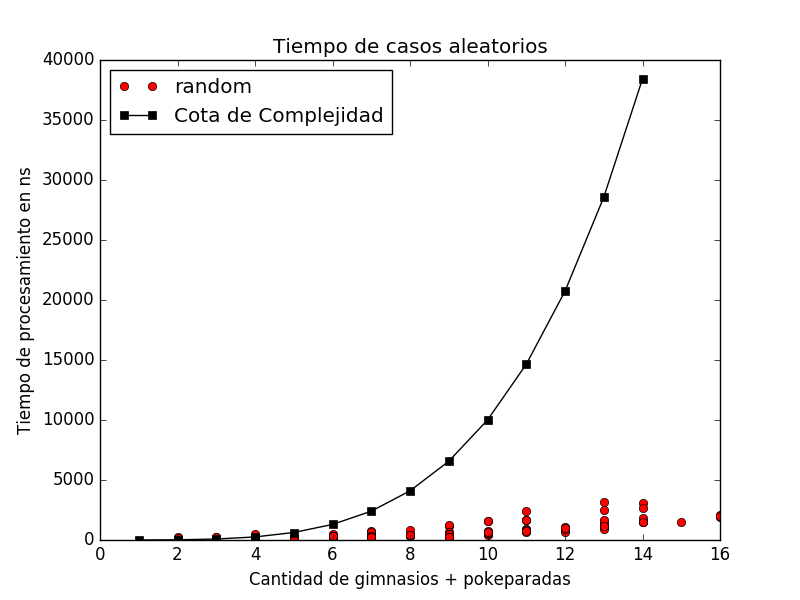
\includegraphics[width=0.7\columnwidth]{imagenes/ejercicio2_exp_random.png}
        \caption{}
      \end{center}
  \end{figure}

     Se puede observar que el tiempo de ejecución de las intancias es bastante mejor que el calculado teóricamente en el peor caso. Esto se debe a que en la mayoría de las instancias el algoritmo no pudo nisiquiera recorrer todos los gimnasios, ya que debido a la configuración de las instancias y el funcionamiento del algoritmo no se podía avanzar a ningún nodo.